\subsection{Flöde vid termisk jämvikt}
\label{sec:steadystatewall}

%To regerenate the figures use /code/pdesolver/generateWallFigApril.m
%with the argument /code/pdesolver/walldata.mat


För att visualisera flödet genom en vägg vid konstant väder och utomhustemperatur görs 
beräkningar med finita elementmetoden och en konstant inomhustemperatur på 
$\unit[20]{^\circ C}$. Utomhusvädret är relativt konstant och är satt till antingen molnig 
eller klart en dag i april då utomhustemperaturen varierar mellan $\unit[6]{^\circ C}$ på natten och $\unit[9]{^\circ C}$ på dagen. Detta har gjorts för en vägg utan isolering och en vägg med 
isolering, se figur~\ref{fig:energyflow_stst}. Den oisolerade väggen består av 
$\unit[0,5]{m}$ tegel och den isolerade har dessutom $\unit[0,1]{m}$ mineralull. 

\begin{figure}[hpbt]
\centering

\subfloat[Energiflöde ut från insidan av en oisolerad vägg en klar dag i april.]{
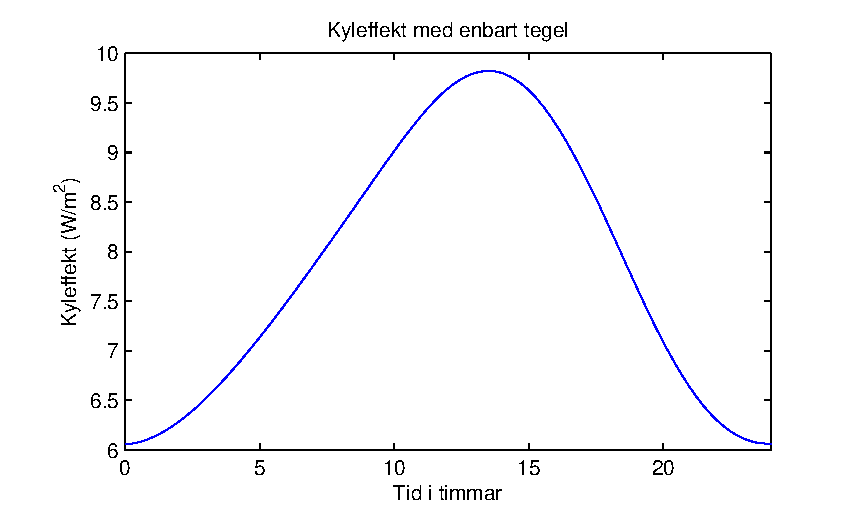
\includegraphics[width=6cm]{images/noinsulationapril.eps}}\vspace{1cm}
\subfloat[Energiflöde ut från insidan av en isolerad vägg en klar dag i april.]{
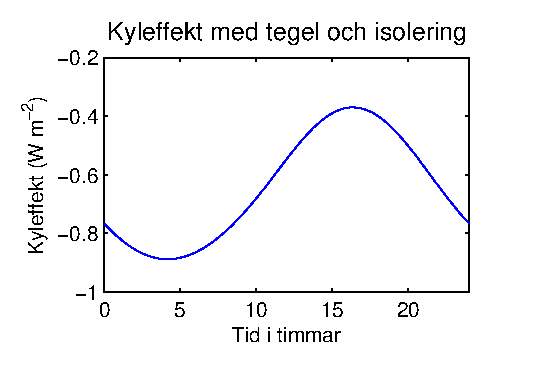
\includegraphics[width=6cm]{images/insulationapril.eps}
}

\subfloat[Energiflöde ut från insidan av en oisolerad vägg en molnig dag i april.]{
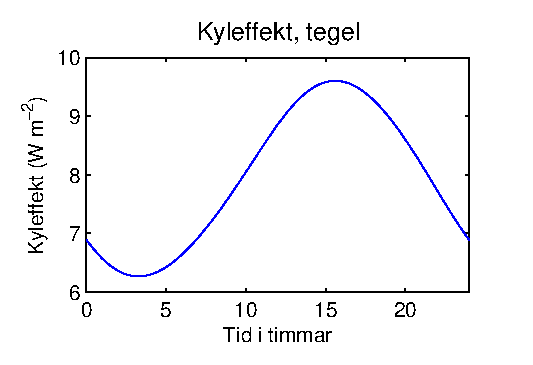
\includegraphics[width=6cm]{images/noinsulationcloud.eps}}\vspace{1cm}
\subfloat[Energiflöde ut från insidan av en isolerad vägg en molnig dag i april.]{
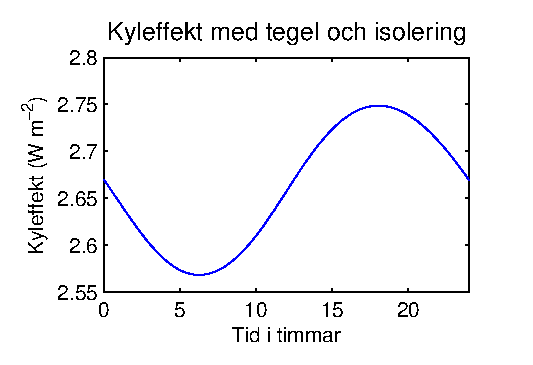
\includegraphics[width=6cm]{images/insulationcloud.eps}
}

\caption{\label{fig:energyflow_stst} Energiflöden ut från insidan av en vägg en dag i mitten av april. Utflöden ut genom väggen betecknas positivt, och inflöden negativt. }
\end{figure}


%RESULTAT ur graferna 
I figur \ref{fig:energyflow_stst} kan vi se att energiflödet genom väggen minskar till 
ungefär en fjärdedel med isolering. Under ett soligt dygn kommer det att flöda värme in i
 fastigheten. På grund av fördröjningen i väggen sker detta främst under natten, 
 och mindre på dagen. Med isolering blir energiflöde mindre och jämnare och inflödet når aldrig över $\unit[1]{W~m^{-2}}$.

Under en molnig dag med samma temperatur varierar energiflödet mellan 7 och 10 
$\unit{W~m^{-2}}$ utan isolering. Med isolering minskar det till att röra sig mellan 2,1 och 2,3 $\unit{W~m^{-2}}$ ut ur 
fastigheten. En isolering innebär en molnig aprildag ett minskat energiutflöde och därmed en minskad 
energiförlust för fastigheten.

Trots att energi flödar in i fastigheten den klara dygnet så flödar ganska mycket energi 
ut ur fastigheten under det molniga dygnet. Göteborg har 1800 soltimmar under ett
 år av de totalt 4380 timmar som solen är över horisonten. Utifrån SMHI:s väderstatistik \cite{SMHIdata}
 kan beräknas att ungefär 37\% av dessa sker under eldningssäsongen, oktober till april. 
 Detta motsvarar ungefär 8\% av dygnets alla timmar. Tyvärr så förlorar fastigheten mer 
 energi än vad den tjänar på att inte isoleras utslaget på hela eldningssäsongen.

Under en fin sommardag kan det också tänkas att fastigheten värms över den önskade 
temperaturen och energi istället måste läggas på kylning. Med en isolering minskas även 
effekten av detta och energiflödena blir mindre och jämnare.

%%%%%%%%%%%%%%%%%%%%%%%%%%%%%%%%%%%%%%%%%%%%
\paragraph{En decemberdag}

Vidare har också energiflödena genom väggen en kall decemberdag undersökts, 
alltså en dag där energiflödena bör bli ganska stora. Detta kan ses som en övre uppskattning på fastighetens energiåtgång. Två fall av
denna dag har undersökts, dels en molning dag och dels en klar dag.

 Temperaturen går från $\unit[-5]{^\circ C}$ på dagen till $\unit[-11]{^\circ C}$. 
 Konvektionskoefficienten har satts till $h=\unit[35]{W~m^{-2}~K^{-1}}$ 
 vilket motsvarar en vindhastighet $\unit[5]{m~s^{-1}}$ parallellt med väggens yta. 
 Beräkningarna är genomförda genom att väggens tvärsnitt approximerats med en stav och sedan behandlats med finita elementmetoden.


\begin{figure}[hpbt]
\centering
\subfloat[Energiflöde ut från insidan av en oisolerad vägg en molnig dag i december.]{
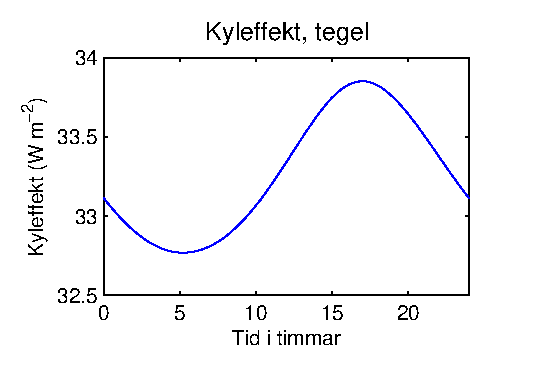
\includegraphics[width=6cm]{images/noinsulationdec.eps}}
\subfloat[Energiflöde ut från insidan av en isolerad vägg en molnig dag i december..]{
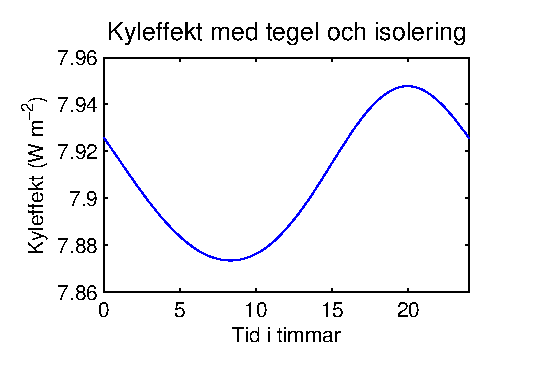
\includegraphics[width=6cm]{images/insulationdec.eps}
}

\subfloat[Energiflöde ut från insidan av en oisolerad vägg en klar dag i december.]{
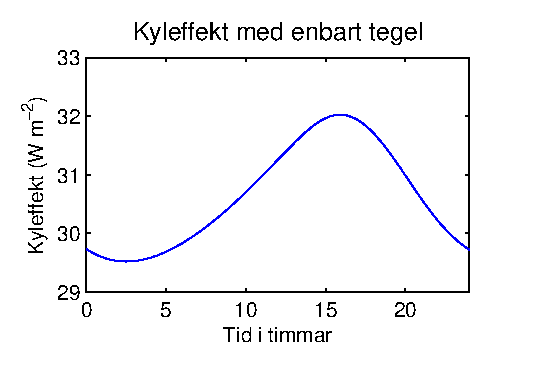
\includegraphics[width=6cm]{images/decsunnoinsulation.eps}
}\vspace{1cm}
\subfloat[Energiflöde ut från insidan av en isolerad vägg en klar dag i december.]{
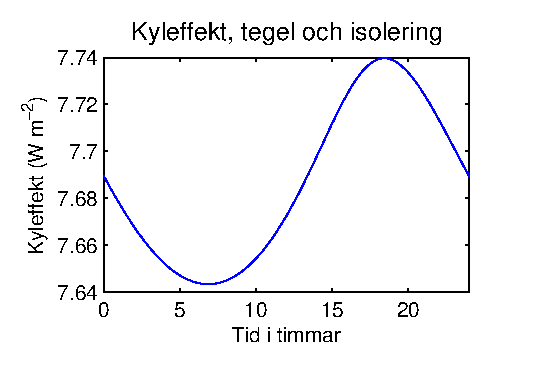
\includegraphics[width=6cm]{images/decsuninsulation.eps}
}

\caption{\label{fig:wall_dec} Energiflöden ut från insidan av en vägg en dag i december Utflöden ut genom väggen betecknas positivt, och inflöden negativt. 
}
\end{figure}

% Resultat
Även i december blir energiflödet genom en isolerad vägg ungefär en fjärdedel av det 
genom en oisolerad vägg, se figur~\ref{fig:wall_dec}. Här minskar det dock från ungefär 33 
till $\unit[7,9]{W~m^{-2}}$ ut ur väggen för den molniga dagen och från ungefär 31 till 7,4 $\unit{W~m^{-2}}$ den soliga dagen. Vi ser också i figurerna att energiflödet också blir 
jämnare med isolering – det varierar med mindre än $\unit[0,1]{W~m^{-2}}$ över dygnet, 
istället för drygt $\unit[1]{W~m^{-2}}$ utan isolering. Det gäller både vid klart och mulet väder. Detta är eftersträvansvärt om en jämn inomhustemperatur önskas. Energiflödet påverkas inte lika mycket av solen på vintern som under den varmare delen av året. En dag i december finns det betydligt mindre att tjäna på att inte isolera och hoppas att solen skiner, jämfört med en dag i april.

%%%% BURSPRÅK %%%%%%%%%%%%%%%%%%%%%%%%%%%%%%%
\paragraph{Burspråket}

Burspråket är inte uppbyggt av tegel, som de andra väggarna, utan av gips, isolering och koppar på spånskiva, se avsnitt~\ref{subsec:walls}. Energiflödet i burspråket visas här för alla fyra fallen: klar och molnig aprildag samt klar och molnig decemberdag.

\begin{figure}[hpbt]
\centering
\subfloat[\label{fig:bursprak_april1} Energiflöde ut från insidan av burspråket en klar dag i april.]{
	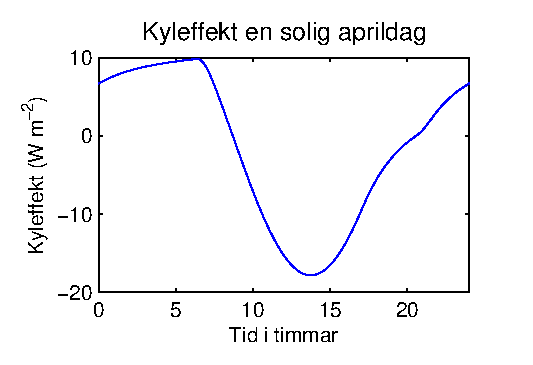
\includegraphics[width=6cm]{images/baysunapril.eps}
}
\subfloat[\label{fig:bursprak_april2} Energiflöde ut från insidan av burspråket en molnig dag i april.]{
	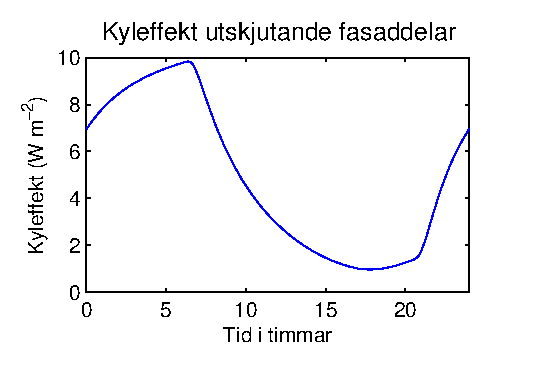
\includegraphics[width=6cm]{images/baynosunapril.eps}
}

\subfloat[\label{fig:bursprak_decsun} Energiflöde ut från insidan av burspråket en klar dag i december.]{
  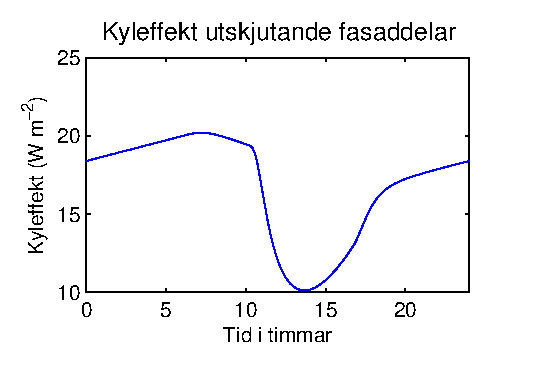
\includegraphics[width=6cm]{images/decsunbay.eps}
}
\subfloat[\label{fig:bursprak_dec} Energiflöde ut från insidan av burspråket en molnig dag i december.]{
	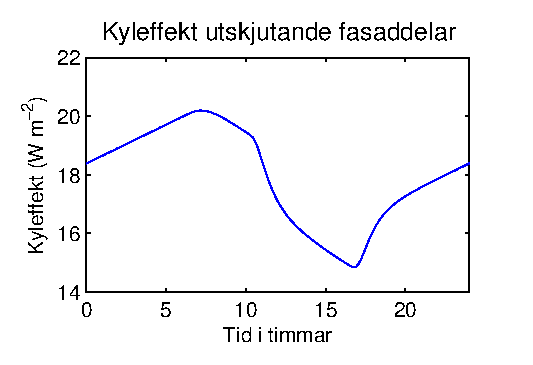
\includegraphics[width=6cm]{images/baynosundec.eps}
}
\caption{\label{fig:bursprak_energi} Energiflöden ut från insidan av en vägg. Utflöden ut genom burspråket betecknas positivt, och inflöden negativt. }
\end{figure}

Genom burspråket ser energiflödet lite annorlunda ut jämfört med det genom tegelväggarna, se figur~\ref{fig:bursprak_energi}. En aprilmorgon innan solen har gått upp når energiflöde sitt maximum med $\unit[10]{W~m^{-2}}$. När solen sedan värmer burspråket börjar energi istället flöda in i byggnaden och en riktigt solig dag är det maximala inflödet nästan $\unit[20]{W~m^{-2}}$, se figur~\ref{fig:bursprak_april1}. En molnig dag stannar det istället på ungefär $\unit[1]{W~m^{-2}}$ ut ur burspråket, se figur~\ref{fig:bursprak_april2}

En molnig dag i december är det betydligt kallare och energiutflödet varierar mellan 15 och $\unit[20]{W~m^{-2}}$, se figur~\ref{fig:bursprak_dec}. En solig decemberdag är det tyvärr inte mycket bättre och kyleffekten är alltid större än $[7,3]\unit{W~m^{-2}}$, se figur~\ref{fig:bursprak_decsun}.
 En intressant detalj är att kyleffekten på burspråket inte alls är sinusformad, på det vis som flödet genom väggarna i figur~\ref{fig:energyflow_stst} och \ref{fig:wall_dec} är. Det beror troligen på att burspråkets väggar är väldigt tunna och reagerar snabbt på förändringar.

%%%%%%%%TAKET%%%%%%%%%%%%%%%%%%%%%%%%%%%%%%%
\paragraph{Taket}

Energiflödet genom taket beräknas på samma sätt som energiflödet genom väggarna. Skillnaden, förutom materialet, är takets vinkel mot solen. I figur~\ref{fig:rooffiguressun} visas energiflödet för en solig april- respektive decemberdag. Eftersom taket lutar har nordsidan och sydsidan olika flöden ty solen skiner olika mycket på de olika lutade ytorna. Figur \ref{fig:rooffigurescloud} visar i sin tur situationen på molniga dagar, då ingen direkt solstrålning faller på taket.



\begin{figure}[hpbt]
\centering
\subfloat[\label{fig:roofaprilsunsouth} Energiflöde ut från insidan av sydsidan av taket en klar dag i april.]{
	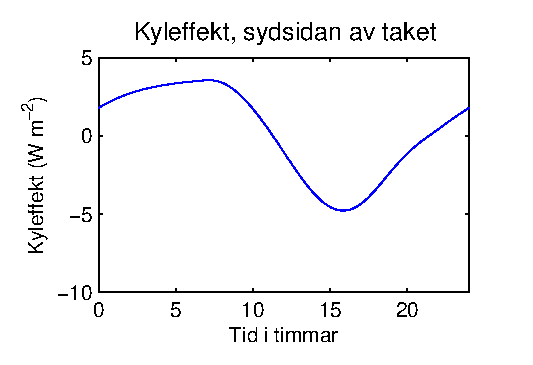
\includegraphics[width=6cm]{images/roofaprilsunsouth.eps}
}
\subfloat[\label{fig:roofaprilsunnorth}Energiflöde ut från insidan av norrsidan av taket en klar dag i april.]{
	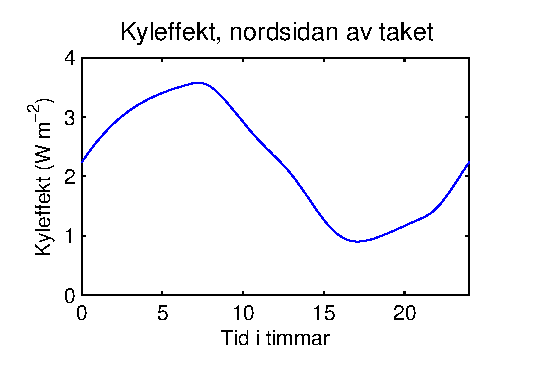
\includegraphics[width=6cm]{images/roofaprilsunnorth.eps}
}

\subfloat[\label{fig:roofdecsunsouth} Energiflöde ut från insidan av sydsidan av taket en klar dag i december.]{
	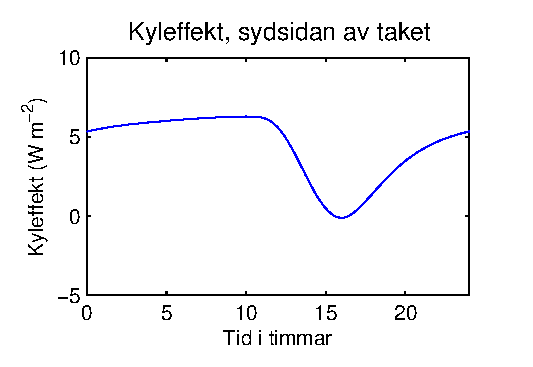
\includegraphics[width=6cm]{images/roofdecsunsouth.eps}
}
\subfloat[\label{fig:roofdecsunnorth} Energiflöde ut från insidan av nordsidan av taket en molnig dag i december.]{
	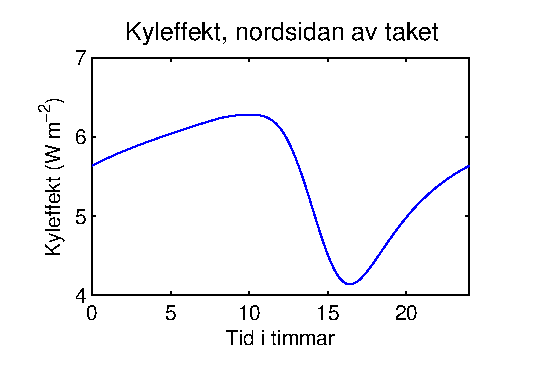
\includegraphics[width=6cm]{images/roofdecsunnorth.eps}
}

\caption{\label{fig:rooffiguressun}Energiflöden ut från insidan av en taket, soliga dagar. Utflöden ut genom taket betecknas positivt, och inflöden negativt. }
\end{figure}

\begin{figure}[hpbt]
\centering
\subfloat[\label{fig:roofaprilnosun} Energiflödet från insidan av taket en molnig aprildag.]{
	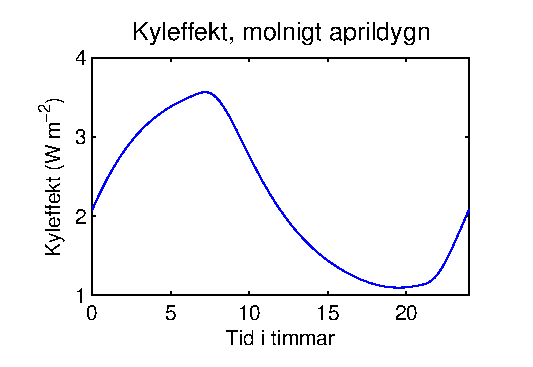
\includegraphics[width=6cm]{images/roofaprilnosun.eps}
}
\subfloat[\label{fig:roofdecnosun} Energiflödet från insidan av taket en molnig decemberdag.]{
	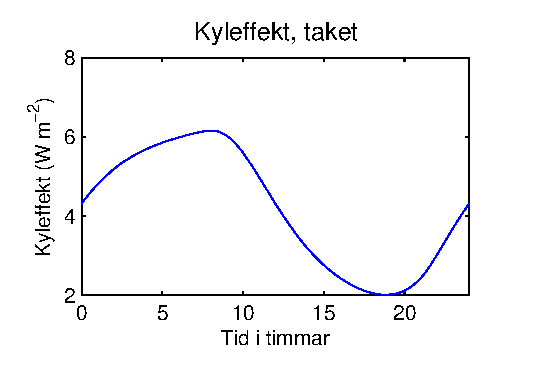
\includegraphics[width=6cm]{images/roofdecnosun.eps}
}

\caption{\label{fig:rooffigurescloud}Energiflöden ut från insidan av en taket, soliga dagar. Utflöden ut genom taket betecknas positivt, och inflöden negativt.}
\end{figure}

Energiflödet genom taket en solig dag i april varierar mellan $\unit[5]{W~m^{-2}}$ in och $\unit[4]{W~m^{-2}}$ ut på sydsidan, se figur~\ref{fig:roofaprilsunsouth}, och mellan 1 och $\unit[3]{W~m^{-2}}$ ut på nordsidan, se figur~\ref{fig:roofaprilsunnorth}. Detta kan vidare jämföras med en molnig aprildag där utflödet varierar ännu mindre, bara mellan 1 och $\unit[3,5]{W~m^{-2}}$, se figur~\ref{fig:roofaprilnosun}. Solen har alltså stor en påverkan på energiflödets variationer. En dag i december är energiutflödet något högre och varierar mellan 6 och $\unit[4]{W~m^{-2}}$, se figur~\ref{fig:roofdecnosun},


%%%%%%%%%%%%%%%%%%%%%%%%%%%%%%%%%%%%%%%%%%%%
